% Mingyu Xia (夏明宇, Westlake ID: 20251202247) Homework #i & #j
\documentclass[11pt]{whatsnote}
\RequirePackage[compat = 1.1.0]{tikz-feynhand}
\setlength \feynhandblobsize {10mm}
\usepackage[natbib, style = phys, biblabel = brackets, sorting = none]{biblatex}
\addbibresource{reference.bib}

\coverset{
  title   = Quantum Many-Body Theory,
  author  = \ttfamily \textsc{Mingyu Xia},
  afill   = PhD @Westlake University,
  date    = November 2025,
  extinfo = {\includegraphics[width = .1\paperwidth]{logos/myhsia_seal}},
  head    = string.pdf,
  clogo   = cat.pdf,
  llogos  = {mouse1.png, mouse2.png,
             mouse4.png, mouse5.png}
}

\begin{document}

\maketitle[violet]
\frontmatter
\tableofcontents
\mainmatter

\include{./context/1_.tex}
% !TeX root = ../main.tex

\chapter{Gaussian Integral}

\section{Free Gaussian Integral}

\[I = \int_{-\infty}^{+\infty} \d x \upe^{-x^2} = \sqrt\pi, ~ I^2 = \pi\]

\subsection{Perturbation expansion of $\mathsf{\int_{-\infty}^{+\infty} \d x \upe^{-x^2-gx^4}}$}

\begin{equation}
  Z(g) = \sum_{n = 0}^\infty \frac{(-g)^n}{n!} \int \d x x^{4n} \upe^{-x^2}
  \label{1.1}
\end{equation}
\begin{equation}
  \int x^{2m}\upe^{-x^2}\d x i
\end{equation}
\emph{Perturbation expansion} is actually divergent: $\lim_{n \to \infty} \ab|\frac{a_{n+1}}{a_n}| \Rightarrow \infty$

The series $Z(g)$ has zero convergence radius.

\section{Feynman Diagram}

\begin{enumerate}
  \item Vertice: $gx^4$
  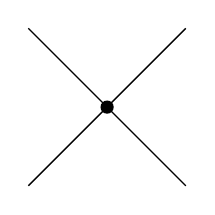
\begin{tikzpicture}[baseline = (o)]
    \begin{feynhand}
    \vertex (a) at (-1,1);
    \vertex (b) at (1,-1);
    \propag [plain] (a) to (b);
    \vertex (c) at (1,1);
    \vertex (d) at (-1,-1);
    \propag [plain] (c) to (d);
    \vertex [dot] (o) at (0,0) {};
    \end{feynhand}
  \end{tikzpicture}
  \item Propagator: $<x$, $x > = \frac12$
  \begin{enumext}[columns = 2]
    \item $n = 1$:
    \[
      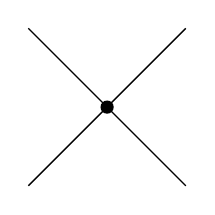
\begin{tikzpicture}[baseline = (o.base)]
        \begin{feynhand}
        \vertex (a) at (-1,1);
        \vertex (b) at (1,-1);
        \propag [plain] (a) to (b);
        \vertex (c) at (1,1);
        \vertex (d) at (-1,-1);
        \propag [plain] (c) to (d);
        \vertex [dot] (o) at (0,0) {};
        \end{feynhand}
      \end{tikzpicture}
      \to
      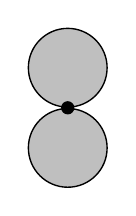
\begin{tikzpicture}[baseline = (o.base)]
        \begin{feynhand}
          \vertex [grayblob, above] (a) at (0,0) {};
          \vertex [grayblob, below] (b) at (0,0) {};
          \vertex [dot] (o) at (0,0) {};
        \end{feynhand}
      \end{tikzpicture}
      +
      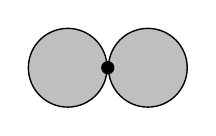
\begin{tikzpicture}[baseline = (o.base)]
        \begin{feynhand}
          \vertex [grayblob, left] (a) at (0,0) {};
          \vertex [grayblob, right] (b) at (0,0) {};
          \vertex [dot] (o) at (0,0) {};
        \end{feynhand}
      \end{tikzpicture}
    \]
    \item $n = 2$:
    \[
      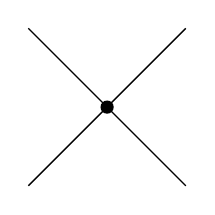
\begin{tikzpicture}[baseline = (o.base)]
        \begin{feynhand}
        \vertex (a) at (-1,1);
        \vertex (b) at (1,-1);
        \propag [plain] (a) to (b);
        \vertex (c) at (1,1);
        \vertex (d) at (-1,-1);
        \propag [plain] (c) to (d);
        \vertex [dot] (o) at (0,0) {};
        \end{feynhand}
      \end{tikzpicture}
      +
      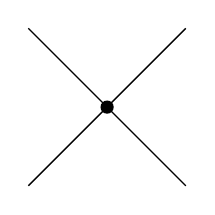
\begin{tikzpicture}[baseline = (o.base)]
        \begin{feynhand}
        \vertex (a) at (-1,1);
        \vertex (b) at (1,-1);
        \propag [plain] (a) to (b);
        \vertex (c) at (1,1);
        \vertex (d) at (-1,-1);
        \propag [plain] (c) to (d);
        \vertex [dot] (o) at (0,0) {};
        \end{feynhand}
      \end{tikzpicture}
      \to
    \]
  \end{enumext}
\end{enumerate}
Symmetry factor.

\section{Finite $n$ still good for $g$-expansion}
\begin{equation}
  Z_\text{exact}(g) = \frac12\sqrt{\frac\pi g} \upe^{1/(8g)} K_{1/4}\ab(\frac{1}{8g})
\end{equation}
$K_{1/4}$ is modified Bessel function.

\begin{tikzpicture}
  \draw [->] (-.5,0) -- (3,0) node [below] {$N$};
  \draw [->] (0,-.5) -- (0,3) node [left, align = right] {error\\$Z_n(g)$ -- $Z_\text{exact}(g)$};
  \draw [dashed, rounded corners] (0,2.5) -- (1.5,.5) -- (3,2.5);
\end{tikzpicture}

Around $N = 13$: it starts going out.

Kondo Problem: to 1 or 2 order.

\noindent\rule{\linewidth}{1pt}

From \eqref{1.1}, we have
\begin{align}
  Z(g)  & = \frac1{g^{1/4}} \int \d y e^{-y^4-y^2/g^{1/2}}\\
        & = \frac1{g^{1/4}} \sum_{m = 0}^\infty \frac{(-1)^m}{m!} \frac{1}{g^{m/2}} \underset{\frac12\frac{\Gamma\left(\frac m2 + \frac14\right)}{g^{m/2} + 1/4}}{\underbrace{\int \d y y^{2m} e^{-y^4}}} \text{(Taylor Expansion)}\\
  \ab|\frac{a_{m+1}}{a_m}| & \to \frac{1}{\sqrt{2g}} \cdot \frac1{\sqrt m} \to 0
\end{align}
Then, $Z(1/g)$ cmverges $(0,+\infty)$

Large $y$, no matter how small $g$ is, $y^4$ term dominates.

\section{Multi-variable Gaussian Integral}

Just means we have found
\begin{equation}
  \int \d x_1 \d x_2 \ldots\d x_N \upe^{-[x][M][x]} =
  \frac12\int \d y_1 \cdots\d y_N \upe^{-[y]u^\dagger Mu[y]}
\end{equation}
\begin{enumext}[columns = 2]
  \item $[x] = (x_1,\ldots,x_N)$
  \item $[M] = (M_{ij})$.
\end{enumext}

Diagonalise $M$: $[x] \to u[y]$, $M \to \pdiagmat[empty = {}]{\ddots, \ddots, \ddots}$,
$u^\dagger Mu = \pdiagmat[empty = {}]{\ddots,\ddots,\ddots}$.

\begin{framed}
  Add interaction:
  \begin{equation}
    \int \d x_1 \ldots \d x_N \upe^{-\sum_{i = 1}^N x_i^4 g}
  \end{equation}
\end{framed}

Consider strong coupling expansion:
\begin{equation}
  \int \d x_1 \cdots \d x_n \upe^{-\sum x_{i1}, x_{i2}, \ldots, x_{in} g_{12}^{34}}
\end{equation}
\begin{equation}
  \int \d y_1 \cdots \d y_N = \upe^{-y^4}
\end{equation}
\include{./context/3_.tex}
\include{./context/4_.tex}
\include{./context/5_.tex}
% !TeX root = ../main.tex

\chapter{More Green's Functions}

\section{Green's function}

\subsection{GFs differential Eqs}

\begin{equation}
  \odv*[2]fx + S(x) f(x) = 0, \qq{or} \hat{\mathcal L} f = 0
\end{equation}
then we can construct $\odv*[2]gx = S(x)$, $f = \int \d x g \cdot S(x)$.

\subsection{GF as propagators in Q.M.}

From the S.E.
\[
  \iu \hbar \pdif t\psi = H\psi
\]
we get the G.F. $G = \braket<x|U|x'>$. To be specific
\begin{equation}
  \ab(\iu\hbar \pdif t + \frac{\hbar^2}{2m}\nabla^2) G_{t,x;t',x'} = \delta(t - t') \delta(x - x')
\end{equation}
which is the EOM, and $G_{t,x;t',x'}$ is the P.I.

\subsection{One particle GF \&  real frequency/real time}

Consider the indicate label $\lambda$, the GF
\begin{equation}
  G_{\lambda\lambda'}
= -\iu \braket<\phi|\mathcal T\psi_\lambda(t) \psi_{\lambda'}^\dagger(t')|\phi>
\end{equation}
where
\begin{equation}
  \mathcal T \hat\psi_\lambda(t) \hat\psi_{\lambda'}^\dagger =
  \begin{cases}
    \psi_\lambda(t) \psi(t'), & t > t'\\
    \pm \psi_\lambda^\dagger(t') \psi_\lambda(t), & t < t'
  \end{cases}
\end{equation}
and the Bosons for $+$ and Fermions for $-$. To combine,
\begin{equation}
  \mathcal T \hat\psi_\lambda(t) \hat\psi_{\lambda'}^\dagger
= \theta(t - t') \psi_\lambda(t) \psi_{\lambda'}^\dagger(t') \pm \theta(t' - t) \psi_{\lambda'}^\dagger(t') \psi_\lambda(t)
\end{equation}
when we take the time derivative,
\begin{equation}
  \begin{aligned}
  \iu\pdif t G & = \delta(t - t') (\psi_\lambda \psi_{\lambda'}^\dagger \mp \psi_{\lambda'}^\dagger \psi_\lambda) + \braket<\mathcal T[\psi, \iu t], \psi_{\lambda'}>\\
  & =
  \begin{cases*}
    \delta(t - t') [\psi_\lambda, \psi_{\lambda'}^\dagger] = \delta(t - t') \delta_{\lambda\lambda'}, & Bosons\\
    \delta(t - t') \{\psi_\lambda, \psi_{\lambda'}^\dagger\} = \delta(t - t') \delta_{\lambda\lambda'}, & Fermions
  \end{cases*} +  \braket<\mathcal T[\psi, \iu t], \psi_{\lambda'}>
  \end{aligned}
\end{equation}
Classically, the commutator is the Poisson bracket $\{\quad\} = \delta_{ij}$.
For bosons and fermions, $\delta_{\lambda\lambda'}$ are all canonical operators,
also exist for many-body operators.

\subsection{Linear response problem: double time -- GFs for arbitrary operators}

\begin{gather}
  G_{\hat A,\hat B}^\text{ret}
= -\iu\theta(t - t') \ab<\braket<[\hat A(t), \hat B(t')]_\pm>>\\
  G_{\hat A,\hat B}^\text{adv}
= +\iu\theta(t' - t) \ab<\braket<[\hat A(t), \hat B(t')]_\pm>>
  G_{\hat A,\hat B}^\text{C} = -\iu\ab<\braket<\mathcal T_\pm(\hat A(t) \hat B(t'))>>
\end{gather}
where $\text C = \text{Causal} = \text{$T$-ordered}$, and
\[
  \ab*<\braket<\hat A(t), \hat B(t')>> = \braket<\Phi|(\hat A(t) - \ab<\hat A(t')>) (\hat B(t') - \ab<\hat B(t')>)|\Phi> = \Tr[\rho \cdots]
\]
and $\braket<A> = \braket<\Phi|A|\Phi>$, also for $B$.

\subsection{Spectral Density of GFs}

\begin{equation}
  S_{AB}(t,t') = \frac1{2\pi}\braket<[A(t), B(t')]_\xi>
\end{equation}
If set $t \to t'$, $G[0] = S_{AB}(t = t')$,
and we can prove the quantities should evolve to
\[
  \braket<A(t)B(t')> = \braket<A(t-t')B(0)>
\]

\subsection{Spectral representation of GF}

\begin{equation}
  H\ket|E_n> = E_n \ket|E_n>,~
  \sum_n \ketbra|E_n><E_n| = \mathbbm 1,~
  \braket<E_n|E_m> = \delta_{nm}
\end{equation}
Take the trace with the exact eigenstates
\begin{equation}
  \begin{aligned}
    \Tr[\upe^{-\beta H} A(t) B(t')] &
  = \sum_{nm} \braket<E_n|\upe^{-\beta H} A(t)|E_n>\braket<E_m|B(t')|E_n>\\
& = \sum \upe^{-\beta E_n} \braket<E_n|A^{(t')}|E_m>\braket<E_m|B^{(t')}|E_m>\\
& = \sum \upe^{-\beta E_n} \upe^{\frac\iu\hbar (E_n-E_m)(t-t')}
    \braket<E_n|\hat A|E_m>\braket<E_m|\hat B|E_n>
  \end{aligned}
\end{equation}
Then we can have
\begin{equation}
  S_{AB}[E] = \sum_{n,m} \delta(E - (E_n - E_m)) (\upe^{\beta E} - \epsilon)
  \braket<E_n|B|E_m>\braket<E_m|A|E_n> \upe^{-\beta E_n}
\end{equation}
For the fourier transformation of the step function
\begin{align*}
  \theta(t - t') & = \frac\iu{2\pi} \int_{-\infty}^{+\infty}
  \d E \frac{\upe^{-\iu E(t-t')}}{E + \iu 0^+},\\
  \theta(t' - t) & = \frac\iu{2\pi} \int_{-\infty}^{+\infty}
  \d E \frac{\upe^{-\iu E(t-t')}}{E + \iu 0^-}
\end{align*}
Then
\begin{gather}
  G[E] = \frac{f_e(E\cdots)}{f_2(E\cdots)} = \frac{f_1(E)}{\prod(E - E_i)} = \sum_i \frac{g_i(E)}{E - E_i + \iu\sgn[E_i]}\\
  f_2(E\cdots) = \sum_n (E^na_n + E^{n-1}a_n \cdots) = \sum_{i=1}^n(E - E_i)
\end{gather}
Then, the Hilbert transformation of the retard/advanced/canonical GF and $S$-matrix can be written as
\begin{align}
  G^\text{ret}(E) & = \int_{-\infty}^{\infty} \d E' \frac{S_{AB}(E')}{E - E' + \iu 0^+},\\
  G^\text{adv}(E) & = \int_{-\infty}^{\infty} \d E' \frac{S_{AB}(E')}{E - E' + \iu 0^-},\\
  G^\text{C}(E) & = \int_{-\infty}^{\infty} \d E' \frac{S_{AB}(E')}{E - E' + \iu\sgn[E'] 0^+},\\
  S_{AB}(E) & = \frac\iu{2\pi} [G_{AB}(E + \iu 0^+) - G_{AB}(E - \iu 0^+)]
= -\frac1\pi \Im[G_{AB}^\text{ret}(E)].
\end{align}

\section{GFs continent}

For arbitrary operator $A$ and $B$, which could be both Fermionic or Boson
\begin{equation}
  \iu G_{AB}^c = -\iu\ab[\theta(t - t') \braket<A(t) B(t')> \pm
    \theta(t' - t) \braket<B(t')A(t)>]
\end{equation}
where $\braket<A(t)B(t')>$ and $\braket<B(t')A(t)>$ is so-called the greater and lesser Green functions: $G^>$, $G^<$, and $[c,c^\dagger]_\xi = 1$.
The retarded/advanced Green function are defined as
\begin{align}
  G_{AB}^\text{ret} & = -\iu\theta(t - t') \braket<[A(t), B(t')]_\xi>\\
  G_{AB}^\text{adv} & = +\iu\theta(t' - t) \braket<[A(t), B(t')]_{-\xi}>
\end{align}
Now the solution will like
\[
  \frac{1}{E - E_i + \iu\sgn(E)}
\]
where $\sgn(E)$ can be $0^+$ (retarded Green function) and $0^-$ (advanced green functioin). The Heaviside function satisfies the Fourier Transformation
\[
  \theta(t - t') = \frac1{2\pi} \int \d x \frac{\upe^{\iu x(t-t')}}{x + \iu 0^+}
\]
If the state $\Phi_0$ is applied to $G^<$, i.e.,
\[
  \braket<\Phi_0|B(t')A(t)|\Phi_0> \to \Tr[\rho A(t)B(t')]
\]
where
\[
  G[t,t'] = G(t - t', 0) = G(0, t - t')
\]
We define
\begin{equation}
  S_{AB}(E) = \braket<A(t)B(t')>
\end{equation}
Then the retarded Green function becomes
\begin{equation}
  G_{AB}^\text{ret}(E) = \int \d E' \frac{S_{AB}(E)}{E - E' + i0^+} \sim \delta(E - E')
\end{equation}
and we can get $S_{AB}(E)$ from the Green function
\begin{equation}
  S_{AB}(E) = \mp\frac1\pi \Im G^\text{ret/adv}
\end{equation}
and $-\frac1\pi \Im(G[c_k, c_k^\dagger]) = A_k(\omega)$.
Typically,
\begin{align}
  S_{AB}(t,t') & = \braket<A(t)B(t')>,\\
  S_{BA}(t,t') & = \braket<B(t')A(t)>,
\end{align}
If one is measuring $k > k_F$, then $\braket<c_k^\dagger, c_k> = 0$,
$\braket<c_k, c_k^\dagger> = 1$; $k < k_F$.
$\braket<S^+(t)S^-(t')>$,
$\braket<S^-(t')S^+(t)>$.

\subsection{Spectral density}

The commutator and anticommutator
\begin{align*}
  S_{AB}^{(-)} & = \braket<\{A(t), B(t')\}>,\\
  S_{AB}^{(+)} & = \braket<[A(t), B(t')]>,
\end{align*}
If we define $\tilde A = A - \braket<A>$, $\tilde B = B - \braket<B>$,
then $S_{AB}^{(+)} = S_{\tilde A\tilde B}^{(+)}$,
\begin{equation}
  S_{AB}^{(\epsilon)}(E) = S_{\tilde A\tilde B}^{(\epsilon)}(E) + (1 - \epsilon) DS(E)
\end{equation}
which is so-called spectral theorem.

Expand the $\tilde A$, $\tilde B$ term
\[
  \braket<\{(A - \braket<A>)(B - \braket<B>)\}> = \braket<\{A,B\}> - 2\braket<A>\braket<B> + \braket<A>\braket<B>
\]
where we can define
\begin{equation}
  D = -2\braket<A>\braket<B> = \frac1Z \sum_{n,m}^{E_n=E_m}\upe^{-\beta E_n}
  \braket<E_n|B|E_m>\braket<E_m|A|E_n>
\end{equation}
We can get the relation between $S$
\[
  S[A,B] = \frac12(S^{(-)} + S^{(+)}), \quad
  S[B,A] = \frac12(S^{(-)}  S^{(+)})
\]
If taking the limit
\[
  \lim_{E\to0}EG^(\epsilon)(E) = (1 - \epsilon) D
\]
Keldysh-formula.

From the EOM of $\tilde G^\pm$
\begin{gather}
  \iu\pdif t \tilde G^{+,c} = \delta(t) \braket<[A,B]> + \Gamma^+ (ee)= \delta(t) \tilde G^{(-)}(t = 0) + \Gamma^+\\
  \iu\pdif t G_{AB}^{-,c} = \delta(t) \braket<\{A,B\}> + \Gamma^-
\end{gather}
The COBS are $\{\hat u^\alpha\}$, where$u^\alpha u^\beta = f^{\alpha\beta}_\gamma u^\gamma$. The commutator
\[
  \braket<[u^\alpha, u^\beta] = a^{\alpha\beta},
  \braket<\{u^\alpha, u^\beta\}> = c^{\alpha\beta}_\gamma u^\gamma>
\]
Since $[\braket<S^+, S^z>] = \braket<S^x>$.

\section{Finite-$T$ Green function \& Matsubara method}

Denote $\braket<\quad>_\text{thermal}$, then acting
\begin{equation}
  \mathcal T \upe^{\iu \int \d t H} \xleftrightarrow{t\leftrightarrow\iu\tau}
  \upe^{-\int_0^\beta H\tau \d\tau}
\end{equation}

Starting from the thermal average
\begin{equation}
  \braket<A(t)B(t')> = \braket<A(t - t')B(0)>
\end{equation}
considering setting $t \to t - \iu\beta$
\[
  Z \tr[\upe^{-\beta H} \upe^{\iu Ht} A \upe^{-\iu Ht} \upe^{+\iu Ht'}B\upe^{-\iu Ht'}]
\]
The trace $\Tr[AB\cdots C]$ is invariant under cyclE. The thermal average
\begin{equation}
     \braket<A(t-\iu\beta)B(t')>_\text{thermal}
  = \Tr[\upe^{-\beta H} \upe^{\iu H(t-\iu\beta)A\upe^{-\iu(i)}}]
  = \Tr[B(t') \upe^{\iu Ht} A \upe^{-\iu Ht} \upe^{-\beta H}]
  = \Tr[\upe^{-\beta H} B(t') A(t)]
\end{equation}
Som we fund that when $t = t' = 0$
\[
  \braket<A(\tau=\beta)B(0)>_\beta = \braket<A(\iu\tau)B(0)>
\]
and we obtain the EOM and solution
\[
  -\pdv*{A(\tau)}\tau = [A(\tau), H], \quad A(\tau) = \upe^{H\tau} A(0) \upe^{-HE}
\]
Sincee
\[
  \theta(\tau) = \begin{cases*}
    1, & if $\tau > 0$\\
    0, & if $\tau < 0$
  \end{cases*}
\]
Then $T_\tau\{A(\tau) B(\tau')\}$.
\[
  \braket<A(t;)B(t')> \Rightarrow \tau,
  G_{AB}^M (\tau,\tau') = -\braket<\mathcal T_\tau(A(\tau, B(\tau')))> = G_{AB}^M (\tau-\tau',0)
\]
\[
  G_{AB}^M (\tau-\tau',0) = \epsilon G_{AB}^M(\tau - \tau' + n\beta, 0)
\]
To proof that,
\begin{proof}
  \begin{equation}
    G_{AB}^M (\tau-\tau',0) = \mathcal EG_{AB}^M(\tau-\tau' + n\beta,0)
  \end{equation}
  then
  \begin{align*}
    G_{AB}^M (\tau-\tau' + \beta,0) &
  = \Tr[\upe^{-\beta H} \upe^{H(\tau-\tau'+\beta)A}
        \upe^{-H(\tau-\tau'+\beta) B}]\\
  & = \Tr[\upe^{-\beta H} B \upe^{H(\tau-\tau') A \upe^{-H(\tau-\tau')}}]
  = G_{AB}^M [B(0) A(\tau-\tau')] = \epsilon G_{AB}^M (\tau-\tau',0)
  \end{align*}
  For boson: periodic; for fermion: antiperiodic.
  Then apply the Fourier transformathon, we have Matsubara freq.
  Then let $E \to \iu E_n$, $E_n = 2m\pi/\beta$, or $E_n = (2n + 1)\pi/\beta$,
  where $\tau\in(-\beta,\beta)$.
  \[
    \int \d\omega \upe^{\iu\omega t} G[\omega] \ldots \Rightarrow
    \sum_{n=-\infty}^{+\infty} \upe^{\iu E_n\tau} G[\iu E_n] (\ldots)
    \Rightarrow \sum_{n=-\infty}^{+\infty} \upe^{\iu E_n\tau} G[E_n]
  \]
  then
  \begin{equation}
    G[E_n] = \int \d E' \frac{S_{AB}(E')}{\iu E_n - E' + \iu0^+}
  \end{equation}
  along the contour
  \[
    \sum_{n=-\infty}^{+\infty} f(\iu E_n) = \oint \d z \frac{1}{\upe^{\beta z}\mp 1} f(z)
  \]
  to calculate the residue, let $\upe^{\beta z = \pm 1}$, then $\tau\to\beta$, we have
  \begin{equation}
    \sum_n \upe^{\iu E_nt} G[\iu E_n]
  = \int \d z \d z' \frac{\upe^{\tau z} S_{AB}(E')}{(\upe^{\beta z} \pm 1) (z - E')}
  = \int \d z \d z' f^\text{BF}(z) \frac{S_{AB}(E')}{(z - E')}\bigg|_{\tau\to\beta}
  \end{equation}
  SPEOM: $G$.
\end{proof}

\section{Examples of GFs}

\begin{example}
  For fermions, the Hamiltonian
  \[
    H = H_0 - \mu N = \sum \epsilon_k c_k^\dagger c_{k\sigma}
  \]
  So the free fermion
  \[
    \ket|\Phi> = \prod_{k<k_F, \epsilon_k < 0} c_{k\sigma}^\dagger \ket|0>
  \]
  then
  \[
  \]
  where $n_k = \theta(k_F - k]$. THen
  \[
    \braket<\Phi|c_{k\sigma}(t) c_{k'\sigma'}^\dagger(t')|\Phi> = \delta_{\sigma\sigma'} \delta_{kk'} \upe^{-\iu\epsilon_k} \braket<\phi|c_{k\sigma}c_{k\sigma}^\dagger|\phi>
    = \delta_{\sigma\sigma'} \delta_{kk'} \upe^{-\iu\epsilon_k(\tau-\tau')} (1 - n_k)
  \]
  So, the Green function
  \[
    G^c(k,t) = -\iu\ab[(1 - n_k)\theta(t) - n_k\theta(-t)]\upe^{-\iu\epsilon_kt}
  = \begin{cases*}
    -\iu\theta(|k| - k_F)\upe^{-\iu\epsilon_k t}, & $t > 0:$ particle\\
    \iu\theta(k_F - |k|)\upe^{-\iu\epsilon_k t}, & $t < 0:$ holes\\
  \end{cases*}
  \]
  From the Fourier transformathon
  \[
    G^c(k,\omega) = -\iu\ab(\frac{\theta(k_1 - k_F)}{\delta-\iu(\omega - \epsilon_k)} - \frac{\theta(k_1 - |k|)}{\delta+\iu(\omega - \epsilon_k)})
    \to
    \frac1{\omega - \epsilon_k + \iu\delta^+\sgn(|k| - k_F)}
  \]
  where $\theta(k_1 - k_F) \sim 1 - n_k$, $\theta(k_f - |k|) \to n$. i.e., the valid for any eigenstate of H
  \begin{equation}
    \iu\pdif t G = \delta(t) + \epsilon G
  \end{equation}
  Then,
  \[
    G^c = \frac1{\omega - \epsilon_k + \iu\delta^+\sgn(\epsilon_k)}
  \]
  $\prod_{k\in(k_1,k_0)} c_k^\dagger\ket|0>$
  \[
    \frac{1-n_k}{\omega - \epsilon_k} + \frac{n_k}{\omega - \epsilon_k} \Rightarrow\frac{1}{\omega - \epsilon_k}
  \]
  From this, we have
  \[
    E = \sum_k \epsilon_k \braket<n_k> \sim \int G \epsilon \d k
  \]
  and then, we can minimize the energy: $\delta E = 0$,
  for $S_{AB}$ and $S_{BA}$.
\end{example}

\begin{example}[Free boson capped]
  \textbf{No BEC}
  The Hamiltonian
  \[
    H = \sum \omega_q b_q^\dagger b_q
  \]
  and the Green functions
  \[
    G[b_q, b_q^\dagger](k,\omega) = \frac{1}{\omega - \omega_q}
  \]
  $G[\phi_q, \Phi_q]$, where $\Phi_q = b_q + b_q^\dagger$.
  \[
    H_0 = \sum_k \epsilon_k b_k^\dagger b_k
  \]
  \textbf{BEC}
  The ground state is
  \[
    \ket|\Psi> = (a_0^\dagger)^N \ket|0>
  \]
  that is called the BEC.
  when $\epsilon_k \to 0$, $N/V = n_0\big|_{L\to\infty, N\to\infty}$.
  The Green function
  \[
    G_0(k,\omega) = G(a_{k:\epsilon_k = 0}, a_k^\dagger) (k,\omega)
  = \underbrace{-\iu(2\pi)^d n_0 \delta(k) \delta(\omega)}_\text{Coherent Part} + \underbrace{\frac1{\omega - \epsilon_k + \iu0^-}}_\text{Incoherent Part}
  \]
  The interaction Hamiltonian
  \[
    H_\text{int} = g\sum_{k,k'} a_k^\dagger a_{-k}^\dagger a_{k'} a_{-k'}
  \]
  When acting on $\ket|\Psi>$, $k' = 0$
  \[
    H_\text{int} \ket|\Psi> \sim
    H_\text{eff, int} = \sum_{k\neq0} g n_0 \ab(a_k^\dagger a_k + \frac12 a_k^\dagger a_{-k}^\dagger + \frac12a_{-k}a_k), \quad
    H_{B,E} = \sum_{k\neq0} \epsilon_k a_k^\dagger a_k
  \]
  When acting on $\bra<\Psi|>$, $k = 0$
  \[
    \bra<\Psi|H_\text{int}
  \]
  then $a_0\ket|\psi_0> \sim \sqrt{n_0}\ket|\Psi_0>$
  In total, $H_B = H_\text{eff, int} + H_{B, E}$.
  Since Bogolinbov transformation
  \[  
  b_k = u_ka_k - v_ka_{-k}^\dagger
  \]
  Then
  \[
    E_k = \sqrt{\epsilon_k(c\epsilon_k + 2gn_0)} \approxeq \sqrt{\frac{k^2}{2\pi}\ab(\frac{k^2}{2\pi} + 2gn_0)} \approxeq |k| \sqrt{gn_0}/m
  \]
  which is so-called Goldstone mode.
  The Green function
  \[
    \iu \pdif t G = \delta + \epsilon_{k_0}G + \braket<[a_{k_{0'}, H_\text{inf}}], a_{k'}^\dagger> \to
    \braket<g\sum_{k,k'} a_k^\dagger a_k a_k \delta_{k,k'}> ...
  \]
  ...
  Bascially we have $H_0 \ket|\psi_0>$,
  by adding $\delta H$, we have
  \[
    G_0 + \delta G \propto \delta H / \propto H_0 \delta\psi
  \]
\end{example}

\section{Free spin wave / magnos}

* Most accurate to know the Hamiltonian of magnetic field: Applied a strong field
  \[
    H_0 = -B \sum_j S_j^z
  \]
  The ground state
  \[
    \ket|\Psi> = \ket|\uparrow\uparrow \cdots>
  \]
  Then
  \[
    \delta H = \sum T_{ij}^+ (S_i^+ S_j^- + S_i^- S_j^+) + \sum J_{ij}^z S_i^z S_j^z
  \]
  Since $[S_i^+, S_j^-] = \delta_{ij} 2\braket<S_i^z>$, $\{S_i^+, S_i^- = 1\}$, $\{S_i^+, S_j^-\} \neq 0$, $[S_i^+, S_i^z] = S_i^+$
  The correlation function
  \begin{multline*}
    \iu \pdif x [S^+, S_{-j}^-] = \delta_{ij}2\braket<S_i^z> \delta(t) + \braket<\underbrace{[S^+, H_0]}_{B\braket<S_i^+, S_f^->}, S_f^->
    + \braket<[S^+, \delta H^+], S^->\\
    + J^2 \braket<S_j^z> \braket<S_i^+, S_f^->
    + J^z \braket<S_i^z> \braket<S_j^+, S_f^->
    + \braket<[S^+, \delta H^+], S^->
    + J_{ij}^+ \braket<2S_i^z; S_j^+; S_f^->
  \end{multline*}
  Then do the Foruier Transform
  \[
    \omega G[S_i^+, S_f^-] \approxeq 2\braket<S^z> + B\braket<S_i^+, S_f^-> + \sum_{\braket<ij>} J_{ij} 2\braket<S_i^z> \braket<S_j^+, S_f^->
  \]
  Acting $\pdif t$, summing over possible spin moments.
  Finally, this can be
  \[
    \omega G[S^+, S^-](k, \omega) = 2\braket<S^z> + BG + 2\braket<S^z> J\tilde \epsilon_k
  \]
  \[
    G \approxeq \frac{2\braket<S^z>}{\omega - B - 2J^+ \epsilon_k}
  \]
  Another:
  \[
    H_0 = \sum_{\braket<ij>}J_{ij}^z S_i^z S_j^z, \quad
    \delta H = \sum J_{ij}^+ (S_i^+ S_j^- + \text{H.c.})
  \]
  If $J^z < 0$, then FM; If $^z > 0$: then AFM.
  \[
    \ket*|\substack{\uparrow \uparrow\\\uparrow \uparrow}>, \quad
    \ket*|\substack{\uparrow \downarrow\\\downarrow \uparrow}>
  \]
  are all the classic type: SSB.
  \begin{framed}
    For Ruanfum SSB
    \[
      H = \sum J \bm S \cdot \bm S, \quad [\rho, H] \neq 0
    \]
  \end{framed}
  \[
    \omega G = 2\braket<S^z> + \sum_{\braket<ij>} J_{ij}^z \braket<S_j^z> G[S_i^+, S_f^-]
  + \sum_{\braket<ij>} J_{ij}^z \braket<S_i^z> G[S_j^+, S_f^-]
  + \sum J^+ 2\braket<S_i^z> G[S_j^+, S_f^-]
  \]
  For FM:
  \[
    \omega G = 2\braket<S^z> + 4J^z \braket<S^z> G + \braket<S^z> J^z \epsilon_k G + \braket<S^z> J^2 \epsilon_k G
  \]
  then
  \[
    \omega G = 2\braket<S^z> + (4J^z \braket<S^z> + (\braket<S^z> J^z + \braket<S^z> J^z)\epsilon_k)F
  \]
  then the Green function is
  \[
    G = \frac{2\braket<S^z>}{\omega - 4J^+ \braket<S^z>} + \epsilon_k J^z (1 + J^z/J^+)
  \]
  so-called renormalization of (effective) mass of magon.

For the anti-ferron $\ket*|\substack{\uparrow \downarrow\\\downarrow \uparrow}>$
\[
  \begin{pmatrix}
    G[S_A^+ S_A^-] & G[S_B^+ S_A^-]\\
    G[S_A^+ S_B^-] & G[S_B^+ S_B^-]
  \end{pmatrix}
\]
Assume $k - k' = nQ$, $Q = (\pi, \pi)$.
\[
  \begin{pmatrix}
    G[k,k] & G{k+Q,k}\\
    G[k,k+Q] & G[k+Q,k+Q]
  \end{pmatrix}
\]
\[
  \omega [G] =
  \begin{pmatrix}
    2\braket<S^z>_A &\\
    & 2\braket<S^z>_B
  \end{pmatrix} +
  \begin{pmatrix}
    J^z\epsilon_k & J^z\epsilon_k\\
    -J^z\epsilon_k & -J^z\epsilon_k
  \end{pmatrix}
\]
where $\epsilon_{k+Q} = -\epsilon_k$.
Eventually we will find that
\[
  \sqrt{\epsilon_k(\epsilon_k + J^z)} \propto k
\]
AFM: Spin-wave.
In the $k$-space, the $\cos k$ will flipped.
For FM: $\epsilon_k \propto k^2$.

Only consider the very simple ground state
$\ket|\Psi>_0$.

$G_{kk} \sim G_{AA}$, $k \in \text{First Brillouin Zone}$
\begin{center}
  \begin{minipage}{.48\linewidth}
    \centering
    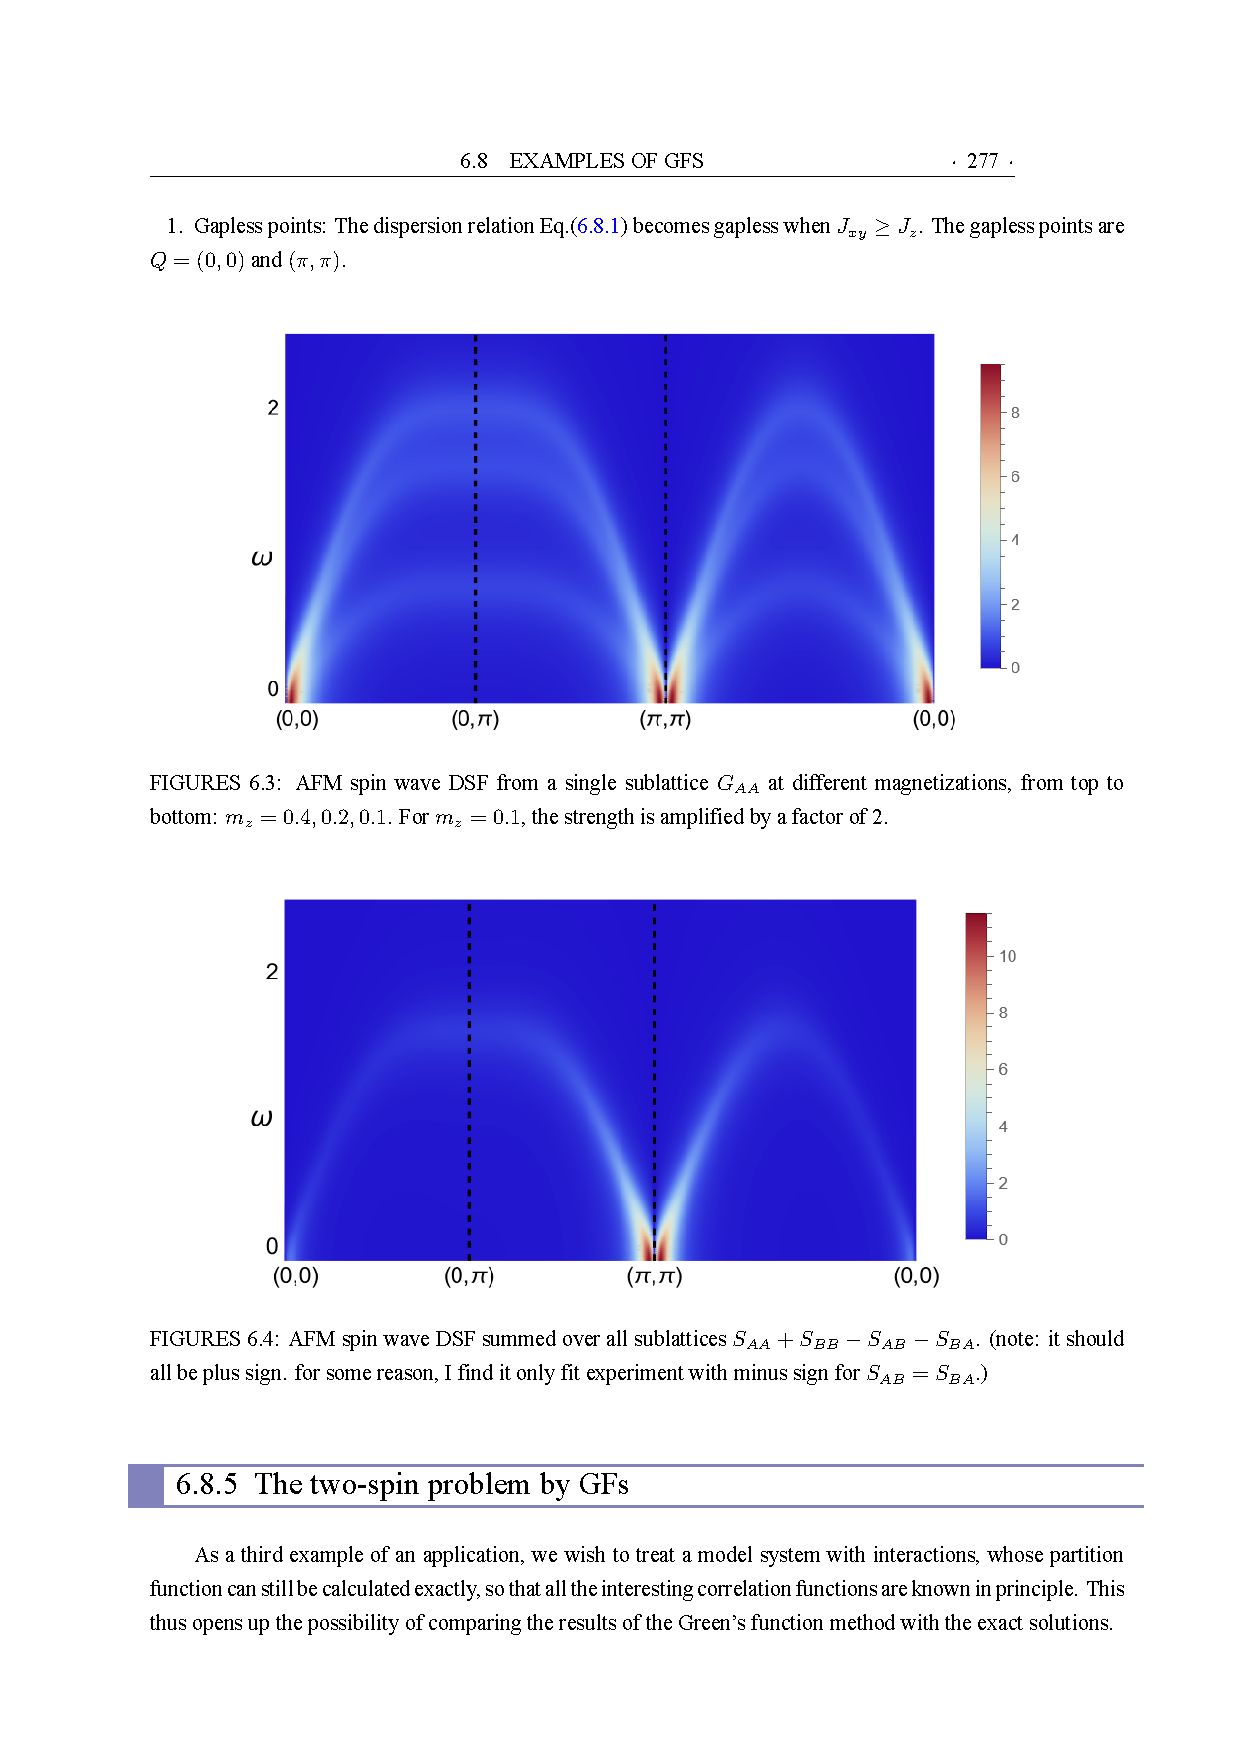
\includegraphics [width = \linewidth, page = 1] {media/GFs}
  \end{minipage}
  \hspace*\fill
  \begin{minipage}{.48\linewidth}
    \centering
    \includegraphics [width = \linewidth, page = 2] {media/GFs}
  \end{minipage}
\end{center}
Roton: liquid \ce{He}.
Roton get deeper during the salivation process.

\section{Quasi-Particle Concept}

\begin{equation}
  \iu\pdif t G_{AB} = \delta(t) \braket<[A,B]>_\xi(t = 0) + \braket<[A,H],B>
= \delta(t) \cdots + \epsilon_k G_0 + \Gamma
\end{equation}
where $\theta(t - t')AB = \theta(t' - t) BA$.
$\braket<[A,H],B>$ is the so-called vertex function $\Gamma = \sum G$, $H = H_0 + V$.
Then, we have the Dyson equation
\begin{equation}
  G_{k\sigma}(E) = G_{k\sigma}^0 + G_k(E)^0 \Sigma(k, E) G_{k\sigma}(E)
\end{equation}
and we can solve the Green function formally as
\begin{equation}
  G_{k\sigma}(E) = \frac1{E - \epsilon_k + \Sigma}, \qq{where}
  G_k^0 = \frac1{E - \epsilon_k}
\end{equation}

\subsection{Self energy}

We assume that $\Sigma$ is the self energy.
\[
  \Sigma = \Re(k, E) + \iu\Im(k, E)
\]
we consider the relation between the advanced and retard Green function
\[
  (G^\text{adv})^* = G^\text{ret}.
\]
In particular,
\begin{equation}
  G_{k\sigma}^\text{ret}(E)
= \frac {(E - \epsilon_k + R) + \iu\identity}
        {(E - \epsilon_k + R)^2 + \iu\identity^2}
\end{equation}
and the equivalent one-electron spectral density
\begin{equation}
  S_{k\sigma}(E) = -\frac1\pi \frac\identity{(E - \epsilon_k + R)^2 + I^2}
\end{equation}

\paragraph{Case A\quad $I = 0$}

Denote $I \to -0^+$. The $\delta$-function becomes
\[
  \delta(E - E_0) = \frac1\pi \lim_{x\to0} \frac x{(E - E_0)^2 + x^2}
\]
Then the equivalent one-electron spectral density becomes
\begin{equation}
  S_k(E) = \delta(E - \epsilon_k + R)
\end{equation}
To get the solution, let the $\delta$-function to be $1$
\[
  E - \epsilon_k + R = 0, \Rightarrow E_i(k)
\]
then, we have
\[
  \delta(E - \epsilon_k + R) = S(E)
= \sum \alpha_i(k) \delta(E - E_i(k)), \qq{and}
  \alpha_i(k) = \ab|1 - \pdv*{k(E)}E|^{-1}
\]
where make use of
\[
  \delta[f(x)] = \sum_i \frac1{f'(x_i)} \delta(x - x_i)
\]

\paragraph{Case B\quad $I \neq 0$}

\begin{align*}
  & \braket<S^+|S^-> \to \braket<\psi(t')|\psi(t)>
  \xlongrightarrow{t-t'\to\infty} \text{Const} \to 0;\\
  & \braket<c|c^\dagger>
\end{align*}
means $\ket|\psi> = S^-\ket|\Psi_0>$ is no longer eigenstate.
Particle will decay.
\[
  |I| \ll |\epsilon_k + R|
\]
Since
\[
  F = \epsilon_k + R
= F(E_i) + (E - E_i)\pdv FE\bigg|_{E=E_i} + \cdots
= E_i + (E - E_i)\pdv FE\bigg|_{E=E_i} + \cdots
\]
Then, the element of the density satisfies
\begin{equation}
  S^{(i)} \approxeq \alpha_i \upe^{-\iu E_i(t-t')}
\end{equation}
and we call the lifetime of quasi-particles $\upe^{-|\alpha \identity||t-t'|} \to \upe^{-|t-t'|/\tau}$, where the lifetime $\tau = 1/|\alpha I|$.
The Real part $\Re[\Sigma]$ and the imaginary part $\Im[\Sigma]$ are \emph{not independent} from each other.
\begin{align}
  \epsilon_k & \approxeq T_0 + \frac{k^2}{2m}\\
  E_i & = T_0 + \frac{k^2}{2m^*}
\end{align}
then, we have
\[
  E_i = T_0 + \frac m{m^*}(\epsilon_k - T_0),
\]
and the fraction of $m$ and $m^*$
\[
  \frac{m}{m^*} = \pdv{E_i(k)}{\epsilon_k} = 1 + \pdv R{\epsilon_k}
= 1 + \pdv R{E_i} \pdv{E_i}k
= \frac{1 - \ab(\pdv R{E_i})_{\epsilon_k}}{1 + \ab(\pdv R{\epsilon_k})_{E_i}}
\]
\include{./context/7_.tex}
% !TeX root = ../main.tex

\chapter{The semi-classical (true) variational approach (WD)}

Starting from the two problems
\begin{center}
  \begin{minipage}{.48\linewidth}
    \centering
    \begin{tikzpicture}
      \draw (0,0) node [left] {$A$}
        to[bend right = 10] (2,-2) node [right] {$B$};
    \end{tikzpicture}
    \[
      \delta \int \d \tau = 0
    \]
  \end{minipage}
  \hspace* \fill
  \begin{minipage}{.48\linewidth}
    \centering
    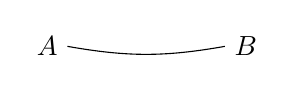
\begin{tikzpicture}
      \draw (0,0) node [left] {$A$}
        to[bend right = 10] (2,0) node [right] {$B$};
    \end{tikzpicture}
    \[
      \delta \int \d l F = 0
    \]
  \end{minipage}
\end{center}
We actually let $\delta \int \d \mathcal L = 0$, i.e., the Euler-Lagrangian EOM.
If it contains the interaction term, then we have the
\emph{Differential-intego-equation}

\section{Variational calculation for free fermions}

\[
  F[n(E)] = \tilde E[n(E)] - TS[n(E)] = \int \d E\phi(E,n)
\]
where $S = -n\ln n - (1 - n)\ln(1 - n)$.
The particle number conservation
\[
  N = \int \d E g(E) n(E), \quad \tilde E = \int \d E E n(E)
\]
We have to minimize the density function
\begin{equation}
  \fdv F{n(E)} \Rightarrow \pdv\phi n = \cdots \Rightarrow
  n^0(E) = \frac1{\upe^{(E-M)/T} + 1}
\end{equation}
also for $\fdv F\mu$.

\subsection{Generic variation around $n^0$}

The energy
\[
  E_0 = \int \frac{\d^ak}{(2\pi)^a} n_k^0 (\epsilon(k))
\]
where $\delta$ expanding some functional (function of functions)
\[
  \delta n_k(\epsilon(k)) = \nu^0(k)
+ \underbrace{\sum_{i = x_i} \pdv n{k_i}
  \bigg|_{n_k^1 \to n^0}}_{\delta(k - k)F,\ \text{The quasi-particle weight}}
  \nu_{k_i}^{(1)} + \frac12 \sum_{i,j} \pdv n{k_i,k_j}
  \underbrace{\nu_{k_ik_j}^{(2)}}_{\pdv n{k_i,k_j}}
\]
To the energy,
\[
  \delta E_0 = \delta \int \frac{\d k}{2\pi} n_k \epsilon_k
= \int \frac{\d k}{2\pi} \epsilon_k \delta n_k
\]
To put $\delta n_k$ into it,
\[
  \fdv En = \fdv*[fun]{\delta E_0 + V(\delta n_k)}n = 0
\]
Now, focus on $T = 0$, then $n_k^{(0)} = \Theta (\epsilon(k) - \mu)$,
$\epsilon_{k_F} - \mu = 0$
\[
  \pdv{n_k^{(0)}}k = \delta(\epsilon(k) - \mu)
  \pdif{k_i} \epsilon \big|_{k\to k_F}
\]
Then, the second derivative
\[
  \pdv{n^{(0)}}{k_i,k_j}
= \ab[\underbrace{\delta (\epsilon - \mu)}_{\delta(k_\bot - k_{F,\bot})}
    \pdif[2]{k_ik_j} \epsilon(k)   \big|_{k\to k_F}
    + \delta'(\epsilon - \mu) \pdif{k_i} \epsilon \pdif{k_j} \big|_{k\to k_F}]
\]
Note that $\delta(k_\bot - k_{F,\bot}) \neq \delta(k - k_r)$, since the shape of
the Fermi surface is arbitrary.
where we can spearate the motion around the Fermi surface into the
parallel and perpendicular terms.
In the simple case single connected Fermi surface
\[
  k_F(\theta) = (k_{r,F}(\theta) \cos\theta, k_{r,F}(\theta) \sin\theta)
\]
where $k_{r,F} (\theta) = k_{r,F_0} + k^0\cos\theta + \cdots$.

Now, we can build the connection between energy and 
\begin{multline}
  \delta E = \int \d \theta \d k_r k_r(\epsilon - \mu)
  (\nu^{(0)} + \delta(k_r - k_{r,F}(\theta)))
  (\pdif{k_r}\epsilon \nu_{k_r} + k_r^{-1} \pdif\theta\epsilon \nu_\theta\\
  + \frac12 \pdif[2]{k_r} \epsilon \nu_{k,k_r} + \cdots) + 
  \frac12\delta'(\epsilon(k) - \mu) (\qquad)
\end{multline}
where
\[
  \nu_{k_r} = \frac{\nu_{k_x}}{\cos\theta} + \frac{\nu_{k_y}}{\sin\theta}, \quad
  \nu_{k_\theta} = -\frac{\nu_{k_x}}{\sin\theta} + \frac{\nu_{k_y}}{\cos\theta}
\]
where the derivative to the $\delta$-function can be expressed as
\[
  \delta'(\epsilon - \mu)
= \pdif\epsilon \delta(k_r(\epsilon) - k_{r,F}(\epsilon))
= (\pdif\epsilon k_r(\epsilon) - \pdif\epsilon \theta(\theta)
  \pdif\theta k_{r,F}) \delta'(k_r - k_{r,F})
\]
and
\[
  \epsilon(k) \Rightarrow k(\epsilon) = \epsilon^{(-1)}(k)
= [(\pdif{k_r}\epsilon)^{-1} + (\pdif\theta\epsilon)^{-1} \pdif\theta k_{r,F}]
  \delta'(\cdots)
\]
The $\delta E$ can have a compact form
\begin{equation}
  \delta E = \delta E^{(0)}
+ \int\d\theta\d k_r k_r \delta^{(T)}(k_r - k_{r,F})
  [(\epsilon - \mu) \pdif{k_r}F + \pdif{k_r}(\epsilon F)]
\end{equation}
where
\[
F =
  [(\pdif{k_r}\epsilon)^{-1} - (\pdif\theta\epsilon)^{-1} \pdif\theta k_{r,F}]
  \frac12 (\pdif{k_r}\epsilon)^2 \nu_{k_r,k_\theta}z + \cdots +
  (\quad)\nu_{k_r,k_r} + (\quad) \nu_{k_\theta k_\theta}
\]

\subsection{Understanding Fermi Liquid: Particle-hole-pairs (LPHPS)}

Bosonization -- 1D case.

The ``vacuum'' state $\ket|\bm 0>_0$, where $c_k\ket|\bm 0> = 0$, with $k > 0$.
The particle number $N$,
\[:\hat A\hat B\hat C: = ABC - \braket<\bm0|ABC|\bm0>\]
For Bosonic, particle-hole-pair operators
\[
  b_q^\dagger = \frac1{\sqrt{n_q}} \sum_{k=-\infty}^\infty c_{k+q}^\dagger c_k,
  \quad b_q = -\frac\iu{\sqrt{n_q}} \sum c_{k-q}^\dagger c_k
\]
where $q = \frac{2\pi}{L} n_q$,
$(b_q^\dagger)^\dagger \to b_q \to b_{-q}^\dagger$.
The particle number
\[
  N_q = b_q^\dagger b_q
\]
If $q > 0$, then without the term $b_{-q}^\dagger$.

The commutator
\[
  [b_q, b_{q'}] = \delta_{q,q'}, \quad
  [b_q^\dagger, b_q'] = \sum\frac1{n1}
  (:c_{k+q-q'}^\dagger c_k - c_{k+q}^\dagger c_{k+q'}:)
= \sum_{k=-\infty}^\infty \frac1{n_q}
  (:c_k^\dagger c_k - c_{k+q}^\dagger c_{k+q}:)
= \delta_{qq'} + \mathcal O(1/k_F)
\]
where $\ket|\bm 0>$ is bosonic ground state
\[
  b_q \ket|\bm N_0> = 0
\]
Look at a typical Fermonic Hamiltonian
\begin{equation}
  \mathcal H = \sum E_p n_p
+ \frac\lambda2 \sum V(q)
  \underbrace{c_{p-q}^\dagger \underbrace{c_{p'+q}^\dagger c_{p'}} c_p}_
  {\frac\lambda2 \sum_{q,k_F,k_F'}V(q)k_{q,k_F}^\dagger b_{q,k_{F'}}}
\end{equation}
The first sum term
\[
  [n_p, b_q^\dagger] = \pm \delta_{p,q} n_q
\]
Then, we obtain the spectral generating algebra
\[
  \sum_{q>0} q b_{q,k_F}^\dagger b_{q,k_F}
+ \frac\lambda2 \sum_{q,k_F,k_F'} b_{q,k_F}' b_{q,k_{F'}}
\equiv \mathcal H_\text{eff}
\]
i.e., the integral equation of $\theta$. The energy
\[
  E(q) \begin{cases}
    \to q/m^*,\\\to \text{Collative hole zero sound}
  \end{cases}
\]
and the matrix form
\[
  \begin{pmatrix}
    q & V(1) & k_fk_{F'}\\
      & \ddots & \ddots \\
    \ddots & & q
  \end{pmatrix}
\]
From $\ket|\bm N_0> \to \ket|\bm\Phi_0>$, $n^0 \to \delta n_p$
jump $Z$ from $Z_1$ to $Z_k$,
\[
  \braket<c^\dagger c^\dagger cc> \to \braket<b_{qk_F}^\dagger b_{qk_{F'}}>
  \propto 1 - Z_k
\]
Identify the \emph{Low energy excitations} (of $\ket|\bm N_0>$).
The interactioin will tend to lower the excited energy.
The interaction will populate the occupy excitations.
If do the canonical
\[
  U\ket|\Phi_0> \Rightarrow (\cdots b^\dagger b^\dagger \cdots) \ket|\bm N_0>
\]

\section{Week Coupling (Canonical) Pertubation Theory}

Starting from the equation of motion of the Green's function
\begin{equation}
  \iu\pdif t G_\epsilon [\underset{s_i^+}{c_i}, \underset{s_j^-}{c_j^\dagger}]
= \delta_{ij}
\end{equation}
where the canonical means that the RHS is a $\delta$-function,
and $[s_i^+, s_j^-] = 2s_i^z\delta_{ij}$.
the operators satisfiy Wick's Theorem
\[
  \{c_i, c_j^\dagger\} = \delta_{ij}, \quad [a_i, a_j^\dagger] = \delta_ij
\]

\subsection{Wick Theorem}

For Gell-Mann-Low, the limitation
\[
  \lim_{\alpha\to0} \frac{u_\alpha^D(0,-\infty)\ket|\eta_0>}
    {\braket<\eta_0|u_\alpha^D(0,-\infty)|\eta_0>}
= \lim_{\alpha\to0} \frac{\ket|\Psi_\alpha^D(0)>}
    {\braket<\eta_0|\Psi_\alpha^D(0)>}
= 
\]
we can convert to the obverse $\braket<A^\text H(t)>$ by computing from the
GML theory
\begin{multline}
  \braket<E_0|A^\text H(t)|E_0>
= \lim_{\alpha\to0} \frac1{\braket<\eta_0|S_\alpha|\eta_0>}
  \sum_{n=0}^\infty \frac1{2^nn!}
  \ab(-\frac\iu\hbar)^n \upe^{-\alpha(|t_1|+\cdots+|t_n|)} \\ \times
  \int_{-\infty}^\infty \d t_1 \cdots \d t_n
  \braket<\eta_0|T_\epsilon
  \ab\{\hat V(t_1)\hat V(t_2) \cdots \hat V(t_n) A^\text H(t)\}|\eta_0>
\end{multline}
where
\[
  V = \frac12 \sum_{\substack{\alpha\beta\\\gamma\delta}}
    \braket<\alpha\beta|\hat V|\gamma\delta>
    a_\alpha^\dagger a_\beta^\dagger a_\gamma a_\delta
\]
The obverse
\[
  \braket<\alpha\beta|\hat V\gamma\delta>
= \braket<\beta\alpha|\hat V|\delta\gamma>
\]
For any observables
\[
  \braket<E_0|A(t) B(t^*) \cdots |E_0>
\]
which can be converted to
\[
  \cdots \int_{-\infty}^\infty \d t_1 \cdots \d t_n
  \braket<\eta_0|
  T_\epsilon\{V(t_1) \cdots V(t_n)
    \underset{a_i(t_i)}A(t) \underset{a_f^\dagger(t_f)}{B(t')} \cdots\}|\eta_0>
\]
To calculate it, consider
\[
  T_\epsilon(O_1(t_1)O_2(t_2)O_3(t_3)O_4(t_4))
\]
which has the order number $4! = 24$.

\subsection{Normal product}

The ``book-keeping'' of counting:
For a given $\ket|\eta_0>$, the fermi wave vector $k_F$, then
\[
  \gamma_k = \begin{cases}
    c_k^\dagger \ket|\eta_0> = 0, & |k| < k_F\\
    c_k \ket|\eta_0> = 0, & |k| > k_F
  \end{cases}
\]
where $\gamma_k\ket|\eta_0> = 0$.
Also for $\gamma_k^\dagger\ket|\eta_0>$.

For $N$-ordering: If we have an arbitrary sequence
\[
  N(\gamma_1 \gamma_2^\dagger \cdots \gamma_n)
  \to (\gamma^+\gamma^+ \cdots | \gamma \gamma \gamma)
\]
where some of the $\gamma$s have $\dagger$.
The normal ordering operator $N$ brings the $\dagger$ to the front.
\[
  \braket<\eta_0|N(\cdots) |\eta_0> = 0
\]
\begin{example}
  $N(\gamma_1\gamma_2^\dagger \gamma_3) = (-1) \gamma_2\gamma_1\gamma_3
= (-1)^2 \gamma_2^\dagger \gamma_3 \gamma_1$.
\end{example}
\begin{example}
  \[c_1c_2c_2^\dagger c_3^\dagger
= (-1)^3c_3^\dagger c_1c_2c_2^\dagger
= (-1)^5c_3^\dagger c_2 c_2^\dagger c_1
= (-1)^5c_3^\dagger (1 - c_2^\dagger c_2)c_1
= (-1)^6 (c_3^\dagger c_2^\dagger c_2 c_1 + (-1)^5(c_3^\dagger\delta_{22}c_1))\]
So, the normal ordering should be
\[
  \underset{\text{operator manipulation}}{N(\cdots)}
= ()c^\dagger c^\dagger \cdots c + c^\dagger \cdots c + () \cdots
\]
\end{example}

\subsection{Contraction}

Define the contraction of two operators
\begin{equation}
  \underbrace{A(t) B(t')}
= T_\epsilon(A(t) B(t')) - \mathcal N(A(t)B(t'))
\end{equation}
The operator identity
\[
  \braket<\eta_0|T_\epsilon(A(t)B(t') - N(A(t)B(t')))|\eta_0>
\]
\subsection{Operator level of ``contraction''}

\begin{example}[Two operators]
  We just look at the RHS of the contraction
  \[
    \underbrace{\gamma(t) \gamma^\dagger(')}
  = T_\epsilon(\gamma(t) \gamma^\dagger(t')) - N(\gamma(t) \gamma^\dagger(t'))
  \]
  On the operator level. Where
  \[
    \theta(t - t') \gamma(t) \gamma^\dagger(t')
  - \theta(t' - t)\gamma^\dagger(t') \gamma(t)
  - [\theta(t - t') + \theta(t' - t)] \gamma^\dagger(t') \gamma(t)
  = \theta(t - t') \gamma(t) \gamma^\dagger(t')
  \]
  Then, we have to define the actual contraction
  \[
    \braket<\eta_0|\underbrace{\gamma \gamma^\dagger}|\eta_0>
  = \iu G^{0,c}[\gamma, \gamma^\dagger]
  \]
\end{example}

Consider 4 time-ordered term
\[
  1\ 2\ 3\ 4:\
  O_1(t_1) O_2(t_2) O_3(t_3) O_3(t_4)
\]
have $4! = 24$ T-ordering: complete permutation of index.
Only look at the two terms
\[
  1234 + 2134 + \cdots
= (12 + 21)34 + T_\epsilon (12)(34)
\xlongequal{\text{Contraction tricks}}
  (\overbrace{12} + N(12)) (34)
\]
So, the observable
\[
  \braket<\eta_0|\quad|\eta_0> = \iu g_{12}^{0c}(34)
+ \braket<\eta_0|N(12)(34)|\eta_0>
\]
So, the two terms gives
\[
  1234 + 2134 \to \iu g_{12}(34), \quad
  1243 + 2143 \to \iu g_{12}(43), \quad
\]
The combines to $\iu g_{12}$ and $\iu g_{34}$,
i.e., $T_\epsilon(\overbrace{12}\overbrace{34})$.
Also for $1324 + 3124$ and $1342 + 3142$, which can be combined into
$T_\epsilon(1234)$. (overbrace 13 and 24).
The LHS have $4!$ terms in total, and we will have $4\times3/2 = 6$ contractions
\[
  g_{12} g_{34} \quad g_{13} g_{24} \quad g_{14} g_{23}
\]
We shall compute
\begin{multline}
  T_\epsilon(123 \cdots 2N)
= N(12\cdots 2N) + \binom{N\text{-product}}{\text{with ONE contraction}}
  N(\underbrace{12}34 \cdots)
+ N(\underbrace{13}24 \cdots 2N) \\
+ \binom{N\text{-product}}{\text{with TWO contraction}}
+ N(\underbrace{12}\underbrace{34}56 \cdots 2N) + \cdots
+ \{\text{total contractions}\}
\end{multline}
\begin{example}[$T_\epsilon(123456)$]
  Apply the result of $1234$
  \[
    T_\epsilon(1234) (56), \quad
    T_\epsilon(C_6^4) \times (C_6^2)
    \to C_6^4 \times \res_{1243} \times (C_6^2)
  \]
  i.e., pick $4$ operators out of $6$.
\end{example}
Do the induction $2n$/$2n + 2$-Wick's
\[
  (\underbrace{12}(34) + N(12)(34)) \cdot
  (\underbrace{56} + N(56)) \to
  \prod_{1, \cdots, 1}^n (\underbrace{i_1 i_2} + N(\\quad))
\]
Together, we have $n$-terms
\[
  1; m \underbrace{} N_{m+1, n}(\quad)
\]
we can put into normal-ordering of arbitrary terms
\[
  \gamma\gamma^\dagger \cdots \gamma^\dagger
= \gamma^\dagger \gamma^\dagger(\delta_{ij} - \gamma^\dagger\gamma)
\]
where we consider $\delta_{ij}$ as one-contruction, and $\ket|\eta_0>$ is the
ground state.

Underlying structure $N(\quad) \ket|\eta_0> = 0$ for Wick's theorem
($\ket|\eta_0>$ Gaussion states).

The canonical algebra
\[
  \{c_i, c_j^\dagger\} = \delta_{ij}, \quad
  \underbrace{\gamma \gamma^\dagger} = T_\epsilon - N(\cdots)
  \to s^2 \Tr(s^+, s^-)
\]
One is canonical algebra, and one is the Gaussion states.
The main idea is to convert $\{s^+, s^-\}$ into canonical bosons:
Schwinger Boson, Maleeev, Pvimakoff.

For $A = \identity$, it becomes
\[
  \fbox{\dots} \Rightarrow \braket<\eta_0|U_\alpha(t,t')|\eta_0>_{t,t'\to\infty}
\]
and $S_\alpha = U_\alpha(+\infty, -\infty)$.
Do the Wick's rotation $t\to\iu\tau$, $S_\alpha \to Z$.
$\braket<\Psi_0|\Psi_0>$ and $\braket<\eta_0|\Psi_D>$.

\section{Feynman Diagram (of what)}

\subsection{$\braket<\eta_0|U|\eta_0>$: Vacuum diagrams}

We rewrite the term into Taylor series form
\begin{equation}
  \braket<\eta_0|U|\eta_0>
= 1 + \sum_{n=1}^\infty \braket<\eta_0|U_\alpha^{(n)}(t,t')|\eta_0>
\end{equation}
For $n = 1$
\[
  V(t_1) = \frac12 \sum_{\substack{kl\\nm}} \nu(kl, nm)
  \int \d t_1' \delta(t_1 -t_1')
    a_k^\dagger(t_1) a_l^\dagger(t_1') a_m(t_1') a_n(t_1)
\]
where the indes is just the matrix element $\braket<kl|v|nm>$.
\begin{align*}
  \braket<u^{(1)}> {=} & \frac12 \sum_{\substack{lk\\mn}} \nu(\cdots)
  \int \d t'\delta(t_1 - t_1')
  \braket<\eta_0|
    T_\epsilon(a_k^\dagger(t_1)a_l^\dagger(t_1')a_m(t_1')a_n(t_1))|\eta_0>\\
{=} & (-\iu G^{0,C}(a_k^\dagger, a_n)[t_1 - t_1])
      (-\iu G^{0,c}(a_0^\dagger, a_m) [t_1' - t_1'])\\
+ & (-1)(-\iu G^{0,c}(a_k^\dagger, a_m)[t_1 - t_i])
    (-\iu G^{0,c} [a_l^\dagger, a_n](t_1' - t_1))
\end{align*}
\begin{center}
  \includegraphics[width = \linewidth]{./media/feynmann1.jpeg}
\end{center}
The operators and the vertices
$
  a_k^\dagger:
  \tikz[baseline]
    { \fill (0,0) circle (.1); \draw [->] (0,0) -- (1,0);} \quad
  a_k:
  \tikz[baseline]
    { \fill (0,0) circle (.1); \draw [<-] (0,0) -- (1,0);}
$
which form through the labeled Feynman diagram.

\subsection{Feynman rules for labeled Feynman diagrams}

\begin{equation}
  V = \frac12 \int \d t_1' \delta(t - t_1') V_{klmn}
      a_k^\dagger(t_1) a_l^\dagger(t_1') a_n(t_1')a_n(t_1)
\end{equation}
\begin{center}
  \includegraphics[width = \linewidth]{./media/feynmann2.jpeg}
\end{center}
For $\braket<lk|\hat V|mn>$, if one switch $\braket<k(L)l(R)|\hat V|n(L)m(R)>$,
then the diagram will be flipped: permuting extremities($L \leftrightarrow R$).
\begin{enumext}[columns = 2]
  \item Vertex i: $\nu(k_i l_i; m_in_i)$
  \item Propagating line:
  \[
    \tikz[baseline]{
      \fill (0,0) coordinate (a) circle (.1) node [below] {$t_i$};
      \fill (1,0) coordinate (b) circle (.1) node [below] {$t_j$};
      \draw (a) to [bend left = 20] (b);
    } \quad
    -\iu G_{k_i}^{0,c} (t_i - t_j) \delta_{k_ik_j}
  \]
  \item Non-propagating line:
  \[
    \tikz[baseline]{
      \node [left] at (-.25,0) {$t_i$};
      \fill (-.25,0) circle (.05);
      \draw [->] (-.25,0) arc (-180:0:.25);
      \draw (0,0) circle (.25);
  } \quad
    G^{0,c}(t_j - t_i)
  \]
  \item $(-1)^S$, $s$\# fermion loop.
  \item Summ order dummy \dots
  \item $\exp(-\alpha(|t_1| + |t_2| + \cdots))$
  \item Integrate $t$ \dots
  \item $\frac1{2^nn!} \ab(-\frac\iu\hbar)^n$
\end{enumext}

\subsection{Unlabeled Feynman diagram \# of labeled diagram $\mathrm{(2\eta)!}$}

\begin{center}
  \includegraphics[width = \linewidth]{./media/feynmann3.jpeg}
\end{center}
we can integrate over
\begin{equation}
  G(t_1 - t_3) G(t_1 - t_2) G(t_2 - t_3)
\end{equation}
in these Feynman diagrams.

\subsection{Remove labels, get right results}

\begin{enumext}
  \item Diagram with same ``topology'' (means classification in math)
  hvae the same value
  \item Given all top. inequ diagram how we count them?
\end{enumext}
\begin{equation}
  \sum_{n_0}\{\text{All contractioin} =\}
\end{equation}
\begin{center}
  \includegraphics[width = \linewidth]{./media/feynmann4.jpeg}
\end{center}

Transformations of $\Gamma \to \Gamma'$,
but leave  it's value unchanged.
\begin{center}
  Symmetry factor.
\end{center}
We put the labes backing: $k$, $l$, $n$, $m$.

\paragraph{Transformation}
Leaves two structures
\begin{enumext}[columns = 2]
  \item Value unchanged
  \item Diff contraction.
\end{enumext}
Two type of transformations ([Ref] Coloman: symmetry factor):
\begin{enumext}[columns = 2]
  \item Permute extremities.
  \item Propagating lines.
\end{enumext}
\begin{center}
  \includegraphics[width = \linewidth]{./media/feynmann5.jpeg}
\end{center}
If we have $n$ vertices and $m$ lines, and this will give
$2^nn!m!$ possibilities.

All these transf leave value unchange, but
\begin{enumext}[columns = 2]
  \item Different contraction (labeled diag)
  \item Same contraction \texttt{->} over counting
\end{enumext}
The sum
\[
  \sum\{\text{All contractions}\}
\]
Symmetry factor: account for overcounting.
The flips come from the transformations
\begin{center}
  \includegraphics[width = \linewidth]{./media/feynmann6.jpeg}
\end{center}

\paragraph{\# Final step}
Obtain the symmetry factor $S$.
\begin{enumext}
  \item All pass: value-inv.transf $G$.
  \item $G_\Gamma$: Transf $\Gamma$ into a deformations (same contraction)
  of itself. Hence, $G_\Gamma$ is sub group of $G$.
  \item $S = \#$ of elements of $G_r$, $S$ must be divisor of $2^nn!m!$.
\end{enumext}

\subsection{Unlabeled Feyman diagram}

Using label permutation to obtain $S$, $\Gamma'$
\[
  G_\Gamma: \mathcal G\{(12), (21)\}
\]
means $1 \to 2$ and $2 \to 1$.
\begin{center}
  \includegraphics[width = \linewidth]{./media/feynmann7.jpeg}
\end{center}
These diagrams have $S = 2$.
\begin{example}
  Two vertices diagram $\mathcal G\{(1234), (3412)\}$. Using label Pertubation:
  $1 \to 3$, $2 \to 4$, $3 \to 1$, $4 \to 2$.
\end{example}
\begin{example}[$(43\ 12) \notin \mathcal G$]
  Diff contraction
\end{example}
\begin{center}
  \includegraphics[width = \linewidth]{./media/feynmann8.jpeg}
\end{center}
\begin{example}
  Compare with two diagrams
  \[
    \mathcal G\{(1234), (3412), (2143), (4321)\} \to S = 4
  \]
  COmbines them Topo ineq.
  \[
    G_\Gamma \to S, \quad
    \cancel{\frac1{2^nn!m!}} \sum\{n||\text{contractionss}\} = \frac1s (\cdots)
  \]
  which cancels by ``All poss value-inv-transf'', for $v = \frac12$.
\end{example}

\printbibliography[title = {\refname\label{chap:bibliography}}]
\newcommand \sectionname {Lecture \#}
\appendix
\sidefoot \thepage
\fancyhead[OL, ER]{Mingyu Xia (Westlake ID: 20251202247)}
\fancyhead[EL]{\sffamily \rightmark}
\fancyhead[OR]{\fontfamily{lmr}\selectfont<<\texttt{\href{mailto:xiamingyu@westlake.edu.cn}{xiamingyu@westlake.edu.cn}}>>}
\addcontentsline{toc}{chapter}{Problem Set}
\renewcommand *\thesection{\sectionname \arabic{section}}
\newweek
\include{./context/week1_[2025-09-02]}
\newweek
\include{./context/week2_[2025-09-09]}
\newweek
\include{./context/week3_[2025-09-16]}
\newweek
\include{./context/week4_[2025-09-23]}
\newweek
\include{./context/week5_[2025-10-09]}
\newweek
\include{./context/week6_[2025-10-16]}
\newweek
\include{./context/week7_[2025-10-22]}
\newweek
\include{./context/week8_[2025-10-28]}
\newweek
\include{./context/week9_[2025-11-04]}
\newweek
% !TeX root = ../main.tex

\section{Homework \#10 [2025-11-11]}

\begin{problem}
  Interpreting the Fermi liquid via a Schrieffer-Wolff transformation.
  We start from a translationally invariant, spin-1/2 fermion system
  \[
    \mathcal H = \mathcal H + \mathcal H_\text{int},
  \]
  where
  \[
    \mathcal H_0 = \sum_{k,\sigma} \epsilon_k c_{k\sigma}^\dagger c_{k\sigma},
    \quad
    \mathcal H_\text{int} = \frac1{2V} \sum_{k,k',q,\sigma,\sigma'} V_{q}
      c_{k+q,\sigma}^\dagger c_{k'-q,\sigma'}^\dagger
      c_{k'\sigma'} c_{k\sigma}.
  \]
  The Fermi sea $\ket|\textsf{FS}>$ is the ground state of $\mathcal H_0$,
  with all states $|k| < k_F$ filled. We assume $V_q$ is weak and smooth
  near $q = 0$.

  To do a canonical transformation for a Fermi liquid state, we want to
  integrate out (cancel out) \textbf{off-shell} excitations. This is different
  from previous cases, where the original interacting terms are canceled out
  entirely. Instead, for a Fermi liquid state, we write $H_\text{int}$
  schematically as
  \[
    \mathcal H_\text{int} = \mathcal H_\text{diag} + H_\text{off},
  \]
  where
  \begin{itemize}
    \item $\mathcal H_\text{diag}$ conserves the number of quasiparticles near
    the Fermi surface (i.e., forward scattering, density-density type).
    \item $\mathcal H_\text{off}$ mixes sectors with different numbers of
    particle-hole pairs (e.g., it creates or destroys particle-hole pairs
    relative to the Fermi sea).
  \end{itemize}
  Formally,
  \[
    \mathcal H_\text{diag} = \frac1{2V}
      \sum_{\substack{k,k',q\\\text{both $k$, $k^\dagger q$ near $k_F$}}}
      V_q c_{k+q}^\dagger c_{k'-q}^\dagger c_{k'} c_k,
  \]
  and $\mathcal H_\text{off}$ is the rest.
  \paragraph{Such separation can be formally done via the semi-classical
    variational method}
  A simplified version is written
  \[
    \mathcal H_\text{diag} = \frac1{2V}
      \sum_{\substack{k,k',q\\
        \text{both $k = |k+q| = |k'-q| = |k'| = k_F$, $q\to0$}}}
      V_q c_{k+q}^\dagger c_{k'-q}^\dagger c_{k'} c_k.
  \]
  So you can see $\mathcal H_\text{off}$ is just $\mathcal H_\text{int}$ with at
  least one momentum that is away from the Fermi surface. We can just keep it in
  the form of $\mathcal H_\text{int}$.

  We choose $\mathcal S$ such that
  \[
    \mathcal H_\text{off} + [\mathcal S, \mathcal H_0] = 0.
  \]
  This means $\mathcal S$ is chosen to cancel the leading-order off-diagonal
  part of $\mathcal H_\text{int}$ under the transformation.

  Then the transformed Hamiltonian becomes
  \[
    \mathcal H' = \mathcal H_0 + \mathcal H_\text{diag}
      + \frac12[\mathcal S, \mathcal H_\text{off}] + \mathcal O(V^3),
  \]
  where the new effective Hamiltonian is block-diagonal up to order $V^2$.

  Constructing $\mathcal S$ explicitly.

  The commutator $[\mathcal S, \mathcal H_0]$ acts as
  \[
    [\mathcal S, \mathcal H_0]
  = \sum_{\alpha\beta} S_{\alpha\beta} (\epsilon_\alpha - \epsilon_\beta)
    c_\alpha^\dagger c_\beta,
  \]
  so to satisfy $[\mathcal S, \mathcal H_0] = -\mathcal H_\text{off}$,
  we can write
  \[
    \mathcal S = \sum_{\alpha\beta}
    \frac{(\mathcal H_\text{off})_{\alpha\beta}}
      {\epsilon_\alpha - \epsilon_\beta}.
  \]
  This is the Schrieffer-Wolff generator, which mixes states differing in
  unperturbed energy. For the present problem, $\mathcal S$ connects a bare
  fermion state $c_{k\alpha}^\dagger \ket|\textsf{FS}>$ to configurations with
  one additional particle-hole pair.
  \paragraph{Now, answer the following questions.}
  \begin{enumext}
    \item Evaluate $[\mathcal S, c_{k\sigma}^\dagger]$;
    \item Transforming the creation operator - ``ressing'' the bare fermion.
    The transformed fermion creation operator is
    \[
      \tilde c_{k\sigma}^\dagger
    = \upe^{\mathcal S} c_{k\sigma}^\dagger \upe^{-\mathcal S}
    = c_{k\sigma}^\dagger + [\mathcal S, c_{k\sigma}^\dagger]
    + \frac12[\mathcal S, [\mathcal S, c_{k\sigma}^\dagger]] + \cdots
    \]
    to the first order in $V$
    \[
      \tilde c_{k\sigma}^\dagger \approx c_{k\sigma}^\dagger
    + [\mathcal S, c_{k\sigma}^\dagger].
    \]
    \item Compute $\tilde c_{k\sigma}^\dagger \ket|\textsf{FS}>$.
    \item Compute quasiparticle weight
    $Z_k \equiv
    |\braket<\textsf{FS}|\tilde c_k\tilde c_k^\dagger|\textsf{FS}>|^2$
    from the canonical transformation.
  \end{enumext}
\end{problem}
\begin{solution}\leavevmode
  \begin{enumext}
    \item Starting from the identity of $\mathcal S$,
    \[
      [\mathcal S, \mathcal H_0] = -\mathcal H_\text{off}.
    \]
    To get the matrix elements of $\mathcal S$, substitute the commutator above
    into the states $\bra<m|$ and $\ket|n>$ ($m \neq n$)
    \[
     -\braket<m|\mathcal H_\text{off}|n>
    = \braket<m|[\mathcal S, \mathcal H_0]|n>
    = \braket<m|\mathcal S|n> E_n - E_m \braket<m|\mathcal S|n>
    = (E_n - E_m) \braket<m|\mathcal S|n>,
    \]
    where $\bra<m|\mathcal H_0 = \bra<m| E_m$
    and $\mathcal H_0\ket|n> = E_n\ket|n>$. Then,
    \[
      \braket<m|\mathcal S|n>
    = \frac{\braket<m|\mathcal H_\text{off}|n>}{E_m - E_n}
    \qq{for} m \neq n,
    \]
    where we set the diagonal elements $\braket<n|\mathcal S|n> = 0$.
    By inserting $\ketbra|m><n|$ to form the identity $\identity$,
    the operator $\mathcal S$ in Dirac notation can be expressed as
    \[
      \mathcal S = \sum_m \sum_n \ket|m>
                   \frac{\braket<m|\mathcal H_\text{off}|n>}{E_m - E_n} \bra<n|
    \]
    So, we can generate $\mathcal S$ from the four operators in
    $\mathcal H_\text{off}$, which is equivalent to the four operators in
    $\mathcal H_\text{int}$ but without the diagonal elements, that is
    \[
      \mathcal S = \sum_{k, k', q, \sigma, \sigma'} S_{kk'q}^{\sigma\sigma'}
        c_{k+q, \sigma}^\dagger c_{k'-q, \sigma'}^\dagger
        c_{k'\sigma'} c_{k\sigma},
    \]
    Then, substitute it into the condition
    $[\mathcal S, \mathcal H_0] = -\mathcal H_\text{off}$ to
    determine $S_{kk'q}^{\sigma\sigma'}$.
    To distinguish the indices, we need to write $\mathcal H_0$ as
    \[
      \mathcal H_0 = \sum_{p, \tau} \epsilon_p c_{p\tau}^\dagger c_{p\tau}
    \]
    Then, the commutator is
    \[
      [\mathcal S, \mathcal H_0]
    = \sum_{k,k',q,\sigma,\sigma'} S_{kk'q}^{\sigma\sigma'}
      \sum_{p,\tau} \epsilon_p [c_{k+q,\sigma}^\dagger c_{k'-q,\sigma'}^\dagger
       c_{k'\sigma'} c_{k\sigma}, c_{p\tau}^\dagger c_{p\tau}].
    \]
    Compute the kernel first
    \begin{multline*}
      [c_{k+q,\sigma}^\dagger c_{k'-q,\sigma'}^\dagger
       c_{k'\sigma'} c_{k\sigma}, c_{p\tau}^\dagger c_{p\tau}]
    = [c_{k+q,\sigma}^\dagger, c_{p\tau}^\dagger c_{p\tau}]
      c_{k'-q,\sigma'}^\dagger c_{k'\sigma'} c_{k\sigma}
    + c_{k+q,\sigma}^\dagger
      [c_{k'-q,\sigma'}^\dagger, c_{p\tau}^\dagger c_{p\tau}]
      c_{k'\sigma'} c_{k\sigma}\\
    + c_{k+q,\sigma}^\dagger c_{k'-q,\sigma'}^\dagger
      [c_{k'\sigma'}, c_{p\tau}^\dagger c_{p\tau}] c_{k\sigma}
    + c_{k+q,\sigma}^\dagger c_{k'-q,\sigma'}^\dagger
      c_{k'\sigma'} [c_{k\sigma}, c_{p\tau}^\dagger c_{p\tau}].
    \end{multline*}
    The four terms
    \begin{enumext}[columns = 2]
      \item $[c_{k+q,\sigma}^\dagger, c_{p\tau}^\dagger c_{p\tau}]
    = -c_{p\tau}^\dagger \delta_{p,k+q} \delta_{\tau,\sigma}$
      \item $[c_{k'-q,\sigma'}^\dagger, c_{p\tau}^\dagger c_{p\tau}]
    = -c_{p\tau}^\dagger \delta_{p,k'-q} \delta_{\tau, \sigma'}$
      \item $[c_{k'\sigma'}, c_{p\tau}^\dagger c_{p\tau}]
    = c_{p\tau} \delta_{k'p} \delta_{\sigma'\tau}$
      \item $[c_{k\sigma}, c_{p\tau}^\dagger c_{p\tau}]
    = c_{p\tau} \delta_{kp} \delta_{\sigma\tau}$
    \end{enumext}
    where we used the anti-commutative properties of the Fermions
    \[
      \{c_{i,j}, c_{i',j'}^\dagger\} = \delta_{i,i'} \delta_{j,j'}, \quad
      \{c_{i,j}, c_{i',j'}\} = \{c_{i,j}, c_{i',j'}\} = 0.
    \]
    Substitute them into the second sum of the commutator
    \begin{align*}
      \sum_{p,\tau} \epsilon_p [c_{k+q,\sigma}^\dagger c_{k'-q,\sigma'}^\dagger
       c_{k'\sigma'} c_{k\sigma}, c_{p\tau}^\dagger c_{p\tau}]
= & - \mathemph{\sum_{p,\tau} \epsilon_p
      c_{p\tau}^\dagger \delta_{p,k+q} \delta_{\tau,\sigma}}
      c_{k'-q,\sigma'}^\dagger c_{k'\sigma'} c_{k\sigma}\\
  & - \mathemph{\sum_{p,\tau} \epsilon_p} c_{k+q,\sigma}^\dagger
      \mathemph[\sum_p]
        {c_{p\tau}^\dagger \delta_{p,k'-q} \delta_{\tau, \sigma'}}
      c_{k'\sigma'} c_{k\sigma}\\
  & + \mathemph{\sum_{p,\tau} \epsilon_p}
      c_{k+q,\sigma}^\dagger c_{k'-q,\sigma'}^\dagger
      \mathemph[\sum_p]
        {c_{p\tau} \delta_{k'p} \delta_{\sigma'\tau}} c_{k\sigma}\\
  & + \mathemph{\sum_{p,\tau} \epsilon_p}
      c_{k+q,\sigma}^\dagger c_{k'-q,\sigma'}^\dagger
      c_{k'\sigma'} \mathemph[\sum_p]{c_{p\tau}
        \delta_{kp} \delta_{\sigma\tau}}.
    \end{align*}
    Due to the sifting property of the $\delta$-function, the second sum of the
    commutator becomes (here take the minus sign out
    since $[\mathcal S, \mathcal H_0] = -\mathcal H_\text{off}$)
    \[
      \sum_{p,\tau} \epsilon_p [c_{k+q,\sigma}^\dagger c_{k'-q,\sigma'}^\dagger
       c_{k'\sigma'} c_{k\sigma}, c_{p\tau}^\dagger c_{p\tau}]
    = -(\epsilon_{k+q} + \epsilon_{k'-q} - \epsilon_{k'} - \epsilon_k)
      c_{k+q,\sigma}^\dagger c_{k'-q,\sigma'}^\dagger c_{k'\sigma'} c_{k\sigma}.
    \]
    Hence, the commutator $[\mathcal S, \mathcal H_0]$ becomes
    \[
      -\mathcal H_\text{off} = [\mathcal S, \mathcal H_0]
    = -\sum_{k,k',q,\sigma,\sigma'} S_{kk'q}^{\sigma\sigma'}
      (\epsilon_{k+q} + \epsilon_{k'-q} - \epsilon_{k'} - \epsilon_k)
      c_{k+q,\sigma}^\dagger c_{k'-q,\sigma'}^\dagger c_{k'\sigma'} c_{k\sigma}
    \]
    To compare with the expression of $\mathcal H_\text{off}$
    \[
      \mathcal H_\text{off} = \frac1{2V}
        \sum_{k,k',q,\sigma,\sigma'}
        V_{q}
        c_{k+q,\sigma}^\dagger c_{k'-q,\sigma'}^\dagger
        c_{k'\sigma'} c_{k\sigma} \qq{where} k\neq k',\ \sigma\neq\sigma'.
    \]
    Then, we arrive at
    \begin{multline*}
      \sum_{k,k',q,\sigma,\sigma'} S_{kk'q}^{\sigma\sigma'}
      c_{k+q,\sigma}^\dagger c_{k'-q,\sigma'}^\dagger c_{k'\sigma'} c_{k\sigma}
    = \mathcal S\\
    = \frac1{2V}
      \sum_{k,k',q,\sigma,\sigma'} \frac{V_{q}}
        {\epsilon_{k+q} + \epsilon_{k'-q} - \epsilon_k - \epsilon_{k'}}
      c_{k+q,\sigma}^\dagger c_{k'-q,\sigma'}^\dagger
      c_{k'\sigma'} c_{k\sigma}.
    \end{multline*}
    This is the second-quantized form of $\mathcal S$.
    Now, calculate the commutator $[\mathcal S, c_{k\sigma}^\dagger]$.
    Calculate the kernel
    \[
      [c_{k+q,\sigma}^\dagger c_{k'-q,\sigma'}^\dagger
       c_{k'\sigma'} c_{k\sigma}, c_{k\sigma}^\dagger]
    \]
    first. To distinguish the indices, we take
    $c_{k\sigma}^\dagger \to c_{p\tau}^\dagger$
    \begin{align*}
      [c_{k+q,\sigma}^\dagger c_{k'-q,\sigma'}^\dagger
       c_{k'\sigma'} c_{k\sigma}, c_{p\tau}^\dagger] &
    = c_{k+q,\sigma}^\dagger c_{k'-q,\sigma'}^\dagger(
      c_{k'\sigma'} \{c_{k\sigma}, c_{p\tau}^\dagger\}
    - \{c_{k'\sigma'}, c_{p\tau}^\dagger\}c_{k\sigma})\\
  & = c_{k+q,\sigma}^\dagger c_{k'-q,\sigma'}^\dagger
      c_{k'\sigma'} \delta_{kp} \delta_{\sigma\tau}
    - c_{k+q,\sigma}^\dagger c_{k'-q,\sigma'}^\dagger
      \delta_{k'p} \delta_{\sigma'\tau} c_{k\sigma},
    \end{align*}
    where $c_{p\tau}^\dagger$ only ``knock'' on $c_{k'\sigma'}$ and
    $c_{k\sigma}$ effectively due to the anti-commutative properties of
    the Fermions. We define the function
    \[
      \Phi(p_1,p_2,q) = \frac1
        {\epsilon_{p_1+q} + \epsilon_{p_2-q} - \epsilon_{p_1} - \epsilon_{p_2}}.
    \]
    Then, the commutator becomes
    \begin{align*}
      [\mathcal S, c_{p\tau}^\dagger] &
    = \sum_{k,k',q,\sigma,\sigma'} \frac{V_q\Phi(k,k',q)}{2V} (
      c_{k+q,\sigma}^\dagger c_{k'-q,\sigma'}^\dagger
      c_{k'\sigma'} \delta_{kp} \delta_{\sigma\tau}
    - c_{k+q,\sigma}^\dagger c_{k'-q,\sigma'}^\dagger
      \delta_{k'p} \delta_{\sigma'\tau} c_{k'\sigma'})\\
  & = \sum_{k',q,\sigma'} \frac{V_q\Phi(p,k',q)}{2V}
      c_{p+q,\tau}^\dagger c_{k'-q,\sigma'}^\dagger c_{k'\sigma'} -
      \sum_{k,q,\sigma} \frac{V_q\Phi(k,p,q)}{2V}
      c_{k+q,\sigma}^\dagger c_{p-q,\tau}^\dagger c_{k,\sigma}.
    \end{align*}
    Swap dummy variables in the second sum: $k \to k'$, $\sigma \to \sigma'$,
    $q \to -q$, and use
    $c_{p+q}^\dagger c_{k'-q}^\dagger = -c_{k'-q}^\dagger c_{p+q}^\dagger$
    \[
      [\mathcal S, c_{p\tau}^\dagger]
    = \sum_{k',q,\sigma'} \frac{V_q\Phi(p,k',q)}{2V}
      c_{p+q,\tau}^\dagger c_{k'-q,\sigma'}^\dagger c_{k'\sigma'} +
      \sum_{k,q,\sigma} \frac{V_{-q}\Phi(k',p,-q)}{2V}
      c_{p+q,\tau}^\dagger c_{k'-q,\sigma'}^\dagger c_{k'\sigma'},
    \]
    where $\Phi(p,k',q) = \Phi(k',p,-q)$. Hence,
    \[
      [\mathcal S, c_{p\tau}^\dagger]
    = \sum_{k',q,\sigma'} \frac{V_q + V_{-q}}{2V}
      \frac{c_{p+q,\tau}^\dagger c_{k'-q,\sigma'}^\dagger c_{k'\sigma'}}
        {\epsilon_{p+q} + \epsilon_{k'-q} - \epsilon_{p} - \epsilon_{k'}}, ~
      [\mathcal S, c_{k\sigma}^\dagger]
    = \sum_{k',q,\sigma'} \frac{V_q + V_{-q}}{2V}
      \frac{c_{k+q,\sigma}^\dagger c_{k'-q,\sigma'}^\dagger c_{k'\sigma'}}
        {\epsilon_{k+q} + \epsilon_{k'-q} - \epsilon_{k} - \epsilon_{k'}}.
    \]
    \item Substitute the result from (a) directly
    \[
      \tilde c_{k\sigma}^\dagger \approx c_{k\sigma}^\dagger
    + \sum_{k',q,\sigma'} \frac{V_q + V_{-q}}{2V}
      \frac{c_{k+q,\sigma}^\dagger c_{k'-q,\sigma'}^\dagger c_{k'\sigma'}}
        {\epsilon_{k+q} + \epsilon_{k'-q} - \epsilon_{k} - \epsilon_{k'}}.
    \]
    \item Substitute the result from (b) directly
    \[
      \tilde c_{k\sigma}^\dagger \ket|\textsf{FS}>
    = c_{k\sigma}^\dagger \ket|\textsf{FS}>
    + \sum_{k',q,\sigma'} \frac{V_q + V_{-q}}{2V}
      \frac{c_{k+q,\sigma}^\dagger c_{k'-q,\sigma'}^\dagger c_{k'\sigma'}}
        {\epsilon_{k+q} + \epsilon_{k'-q} - \epsilon_{k} - \epsilon_{k'}}.
      \ket|\textsf{FS}>
    \]
    \item Evaluate the overlap
    $\bra<\textsf{FS}|c_{k}\tilde c_{k}^\dagger\ket|\textsf{FS}>$ term by term
    \begin{enumext}
      \item The zeroth order $\mathcal O(V^0)$
      \[
        \braket<\textsf{FS}|c_kc_k^\dagger|\textsf{FS}> = 1.
      \]
      Here assume $|k| > k_F$, so $c_{k} c_{k}^\dagger = 1$ in the Fermi sea.
      \item Denote the operator
      \[
        \chi_k \equiv [\mathcal S, c_k^\dagger].
      \]
      The first order $\mathcal O(V^1)$
      \[
        \bra<\textsf{FS}|c_{k} \chi_k \ket|\textsf{FS}>
      = \braket<\textsf{FS}|c_{k} [\mathcal S, c_{k}^\dagger]|\textsf{FS}> = 0,
      \]
      where $\chi_k$ creates a \emph{two-particle, one-hole state} relative to
      the Fermi sea. Applying $c_k$ still leaves a net excitation, and the
      matrix element vanishes since the states are orthogonal
      ($\mathcal{S}$ is off-diagonal).
      \item The second order $\mathcal O(V^2)$
      \[
        \frac12 \braket<\textsf{FS}|c_{k} [\mathcal S, \chi_k]|\textsf{FS}>
      = \frac12 \braket<\textsf{FS}|
          c_{k} [\mathcal S, [\mathcal S, c_{k}^\dagger]]|\textsf{FS}>
      = -\frac12 \bra<\textsf{FS}| \chi_k^\dagger \chi_k \ket|\textsf{FS}>
      = -\frac12 |\chi_k \ket|\textsf{FS}>|^2.
      \]
      Since the generator $\mathcal{S}$ is anti-Hermitian
      ($\mathcal{S}^\dagger = -\mathcal{S}$), the second-order projection
      simplifies to $-\frac12 \braket<\chi_k^\dagger \chi_k>_{\text{FS}}$.
      Substituting the explicit form of $\chi_k$ into the weight, we obtain
      \[
        Z_k = 1 - \frac1{4V^2} \sum_{k',q,\sigma'}
          \frac{|V_q + V_{-q}|
          \theta(k_F - |k'|) \theta(|k + q| - k_F) \theta(|k' - q| - k_F)}
            {(\epsilon_{k+q} + \epsilon_{k'-q}
            - \epsilon_{k} - \epsilon_{k'})^2} < 1,
      \]
      which brings a quasiparticle weight less than $1$.
    \end{enumext}
  \end{enumext}
\end{solution}

\end{document}